\chapter[Brief History of Radiative Heat Transfer][Brief History of Radiative Heat Transfer]{Brief History of Radiative Heat Transfer}
%
\section{Introduction and History}
%
In some sense, the theory of radiative heat transfer is complete, but in a broader sense, there remains far more work to be done. From an engineering perspective, radiative heat transfer between pairs of objects has long been considered a matter of computing view factors and emissivities. Those quantities may then be plugged into the Stefan-Boltzmann law or, for more complicated thermal systems, a linear system determined by Gebhart factors or thermal circuits, to compute energy exchange.\cite{Howell2011} The aforementioned approach to characterizing thermal radiation was enabled by Max Planck at the start of the 20th century when he proposed his blackbody law.\cite{Planck1959} Blackbodies are hypothetical objects which absorb all radiation incident upon their surfaces. By Kirchhoff's law, a perfect absorber like a blackbody is also a perfect emitter.\cite{Kirchhoff1860} Thus, blackbodies should represent an upper bound on the amount of energy which may be exchanged between objects radiatively.

Fast-forward nearly 60 years and the first signs that Planck's law might not tell the whole story started to appear. In 1953, in the Soviet Union, Dr. Sergei Rytov published work connecting electric fluctuations and thermal radiation, which allowed radiation heat transfer to be treated rigorously under the framework of Maxwell's equations using the fluctuation-dissipation theorem.\cite{Rytov1953} His work remained largely unnoticed in the western world until 1959 when it was translated to English.\cite{Rytov1959} Just two years later, a report was published in the United States predicting super-Planckian radiative energy transfer (above that predicted for blackbodies) could occur between the layers of radiation shields in spacecraft.\cite{Emslie1961} This anomalous behavior was attributed to two factors occurring within the vacuum gap separating layers of shielding: interference of propagating waves and tunneling of evanescent waves. Later in that decade, pioneering work\cite{Cravalho1967, Boehm1970, Domoto1970} in the research group of Professor Chang-lin Tien at the University of California, Berkeley helped improve the theoretical predictions predictions made in Ref. \citenum{Emslie1961}.

The final nails in the coffin for the completeness of Planck's theory came in 1970 and 1971. In 1970, further work from Professor Tien's group experimentally confirmed super-Planckian emission by taking measurements at cryogenic temperatures;\cite{Domoto1970a} details of their apparatus and some preliminary results were published in 1968.\cite{Cravalho1968} And in 1971, Polder and Van Hove presented the first correct general formulation of what would eventually be called near-field radiative heat transfer (NFRHT).\cite{Polder1971} Polder and Van Hove built upon the work of Rytov and used the fluctuation-dissipation theorem to predict NFRHT between two semi-infinite half-spaces separated by a vacuum gap to unequivocally show that the contributions of evanescent waves tunneling through the gap could result in heat transfer rates which exceeded Planck's blackbody law by several orders of magnitude. This effectively opened the door to a number of new technologies such as contactless thermal management,\cite{Guha2012} heat-assisted magnetic recording,\cite{Challener2009} thermal diodes,\cite{Otey2010, Iizuka2012} thermophotovoltaics,\cite{Narayanaswamy2003, Francoeur2011b} and thermal antennae,\cite{Greffet2002} just to name a few.

As time passes and technology advances, these formerly fringe cases of anomalous behavior are becoming increasingly common in real world applications, as advances in microelectromechanical systems (MEMS) technology have put thermal systems, such as the two closely-spaced planar surfaces Polder and Van Hove investigated, in the sights of working engineers. The engineering perspective on thermal radiation needs to change accordingly.

\section{Limitations of Classical Radiative Heat Transfer}
%
By all accounts, classical radiative transfer (CRT) is an incredibly successful theory for predicting radiative heat transfer in most everyday circumstances. So how is it possible that its predictions could be off by orders of magnitude in the near-field? The answer lies in Planck's own words. In the introduction to his text \textit{The Theory of Heat Radiation},\cite{Planck1959} Planck assumed that ``the linear dimensions of all parts of space considered, as well as the radii of curvature of all surfaces under consideration, are large compared with the wave lengths of the rays considered.'' In stating this, he himself acknowledged that his approximation would not account for diffractive effects. Using CRT in scenarios with characteristic lengths comparable to the thermal wavelength (approximately 10 \si{\micro\meter} at room temperature) is akin to applying Newtonian gravity to objects in the vicinity of a black hole: it is a limiting case of a larger, more complicated reality. That begs a fundamental question, under what conditions is CRT valid? At least three conditions must be met:
%
\begin{enumerate}
	\item All separation gaps between objects must be greater much than the thermal wavelength (negligible evanescent wave contributions and coherent interference).
	\item All dimensions of objects must be much greater than the thermal wavelength (negligible diffraction).
	\item All objects must emit radiation diffusely.
\end{enumerate}


\section{Near-Field Radiative Heat Transfer}
%
The seminal work by Polder and Van Hove\cite{Polder1971} helped launch NFRHT as a field of study. As is seen in Fig. \ref{fig:Polder1971Citations}, there was a lag between the publication of Ref. \citenum{Polder1971} in 1971 and NFRHT taking off. This is likely due to the exponential rise of computational power catching up to the numerical needs of their work. The heavy use of computational resources is a common feature of many NFRHT theoretical works, and remains a problem to this day. But since the explosive growth in computing capacity in the mid-1990s, the citations to their work, which I use as a proxy for the field itself, have grown dramatically.

NFRHT has been the subject of several recent reviews.\cite{Joulain2005, Volokitin2007, Basu2009, Shen2013, Song2015, Edalatpour2016a, Greffet2017, Boriskina2017, Cuevas2018} In this section, I will cover recent advances in the theory and experimental measurement of NFRHT. I will use an inclusive definition of NFRHT, which considers any form of radiative transfer that violates one of the validity conditions of CRT.


\subsection{Exact Theoretical Frameworks}
%
\begin{figure}
\centering
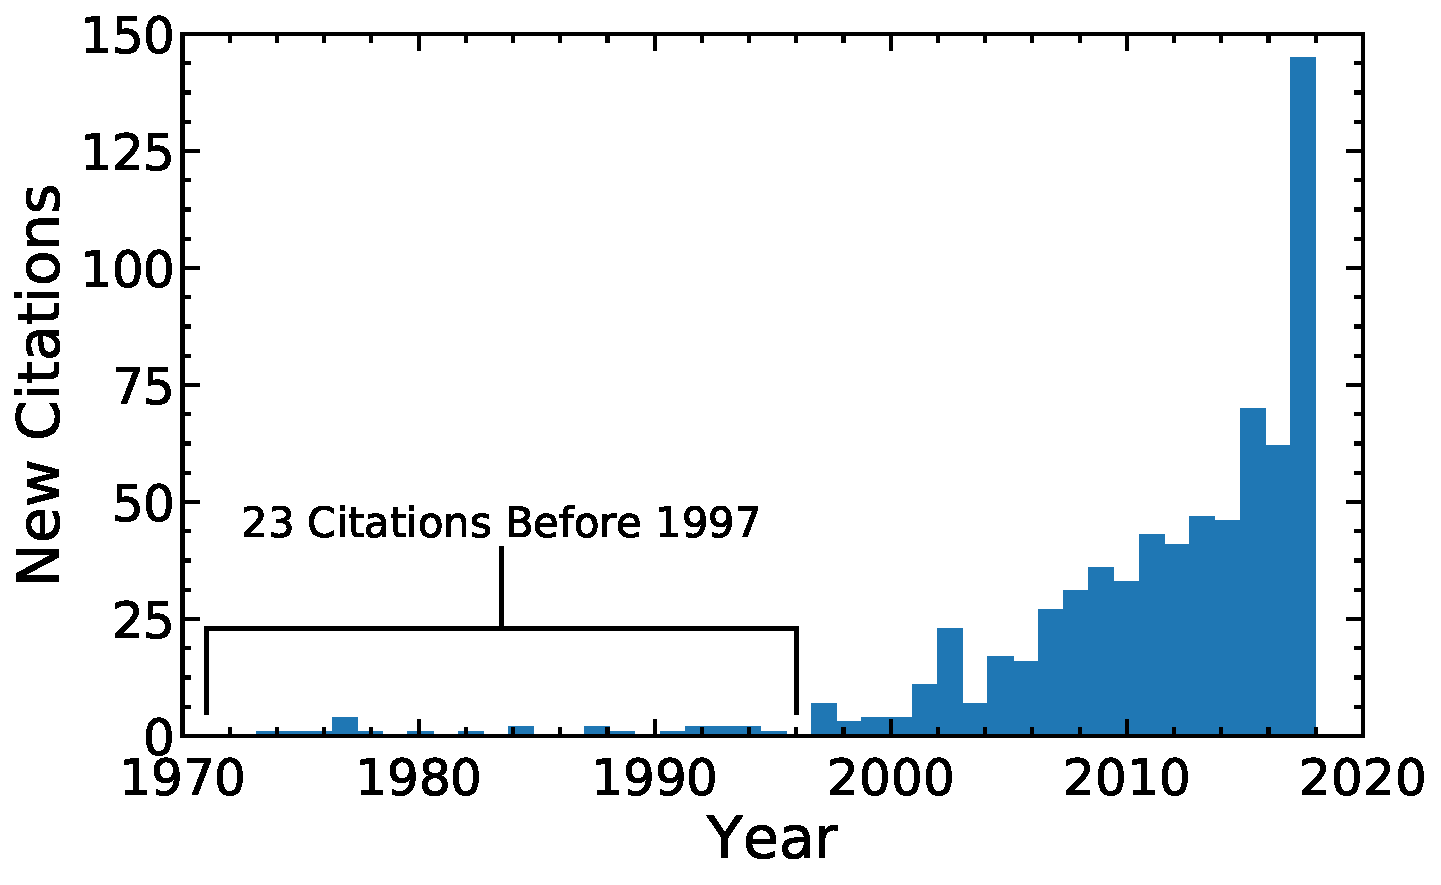
\includegraphics[width=0.8\textwidth]{./Figures/Polder1971Citations.pdf}
\caption{Timeline of citations of Polder and Van Hove's seminal work.\cite{Polder1971}}
\label{fig:Polder1971Citations}
\end{figure}
%
Polder and Van Hove's solution to NFRHT between half-spaces belongs to a class of solutions which are numerically exact for isotropic linear media. That is to say, no theoretical simplifications are required to derive their results and their method converges to the exact value of heat transfer in the correct numerical limit (such as increasing the number of terms in a truncated infinite sum or increasing the density of a mesh). The most common numerically exact methods involve dyadic Green's functions (DGFs),\cite{Joulain2005, Volokitin2007, Francoeur2008, Narayanaswamy2013a} spectral densities,\cite{Kruger2012} fluctuating surface currents/boundary element methods (BEM),\cite{Rodriguez2012} or thermal discrete dipole approximations (T-DDA),\cite{Edalatpour2014} each with its own advantages and limitations. These methods can again be broken into two classes of solutions: meshed and meshless solutions. DGF and spectral density solutions are most commonly meshless. They are best applied to geometries such as spheres, cylinders, and planes which have convenient bases in which to express eigenfunction expansions. BEM and T-DDA typically require surface and volume meshing, respectively. Their great advantage is that they are easily applied to arbitrary geometries; however, their computational time is often significantly greater than their meshless cousins. 

Despite having a number of theoretical frameworks to choose from, the frameworks themselves lack the immediately apparent insight that CRT can provide; their governing formulas are very abstract. To that end, a great deal of research has been directed towards determining explicit formulas for heat transfer in experimentally important thermal systems. Certain problems are best attacked using DGF and spectral density methods such as NFRHT in plane-plane, \cite{Polder1971} sphere-sphere, \cite{Narayanaswamy2008, Mackowski2008, Kruger2012, Czapla2017} and sphere-plane \cite{Kruger2011, Otey2011} configurations, where the electromagnetic fields are easily described by vector wave eigenfunction expansions. Thermal systems which do not yield to those methods often require meshed methods, such as BEM and T-DDA. Those methods have allowed investigations of cone-plane \cite{Rodriguez2013, Edalatpour2016} and cube-cube \cite{Edalatpour2014} configurations, among others. See Fig. \ref{fig:ExactMethods} for examples from the literature. In all cases presented, the characteristic lengths of at least one object were less than the thermal wavelength. 

\begin{figure}
\centering
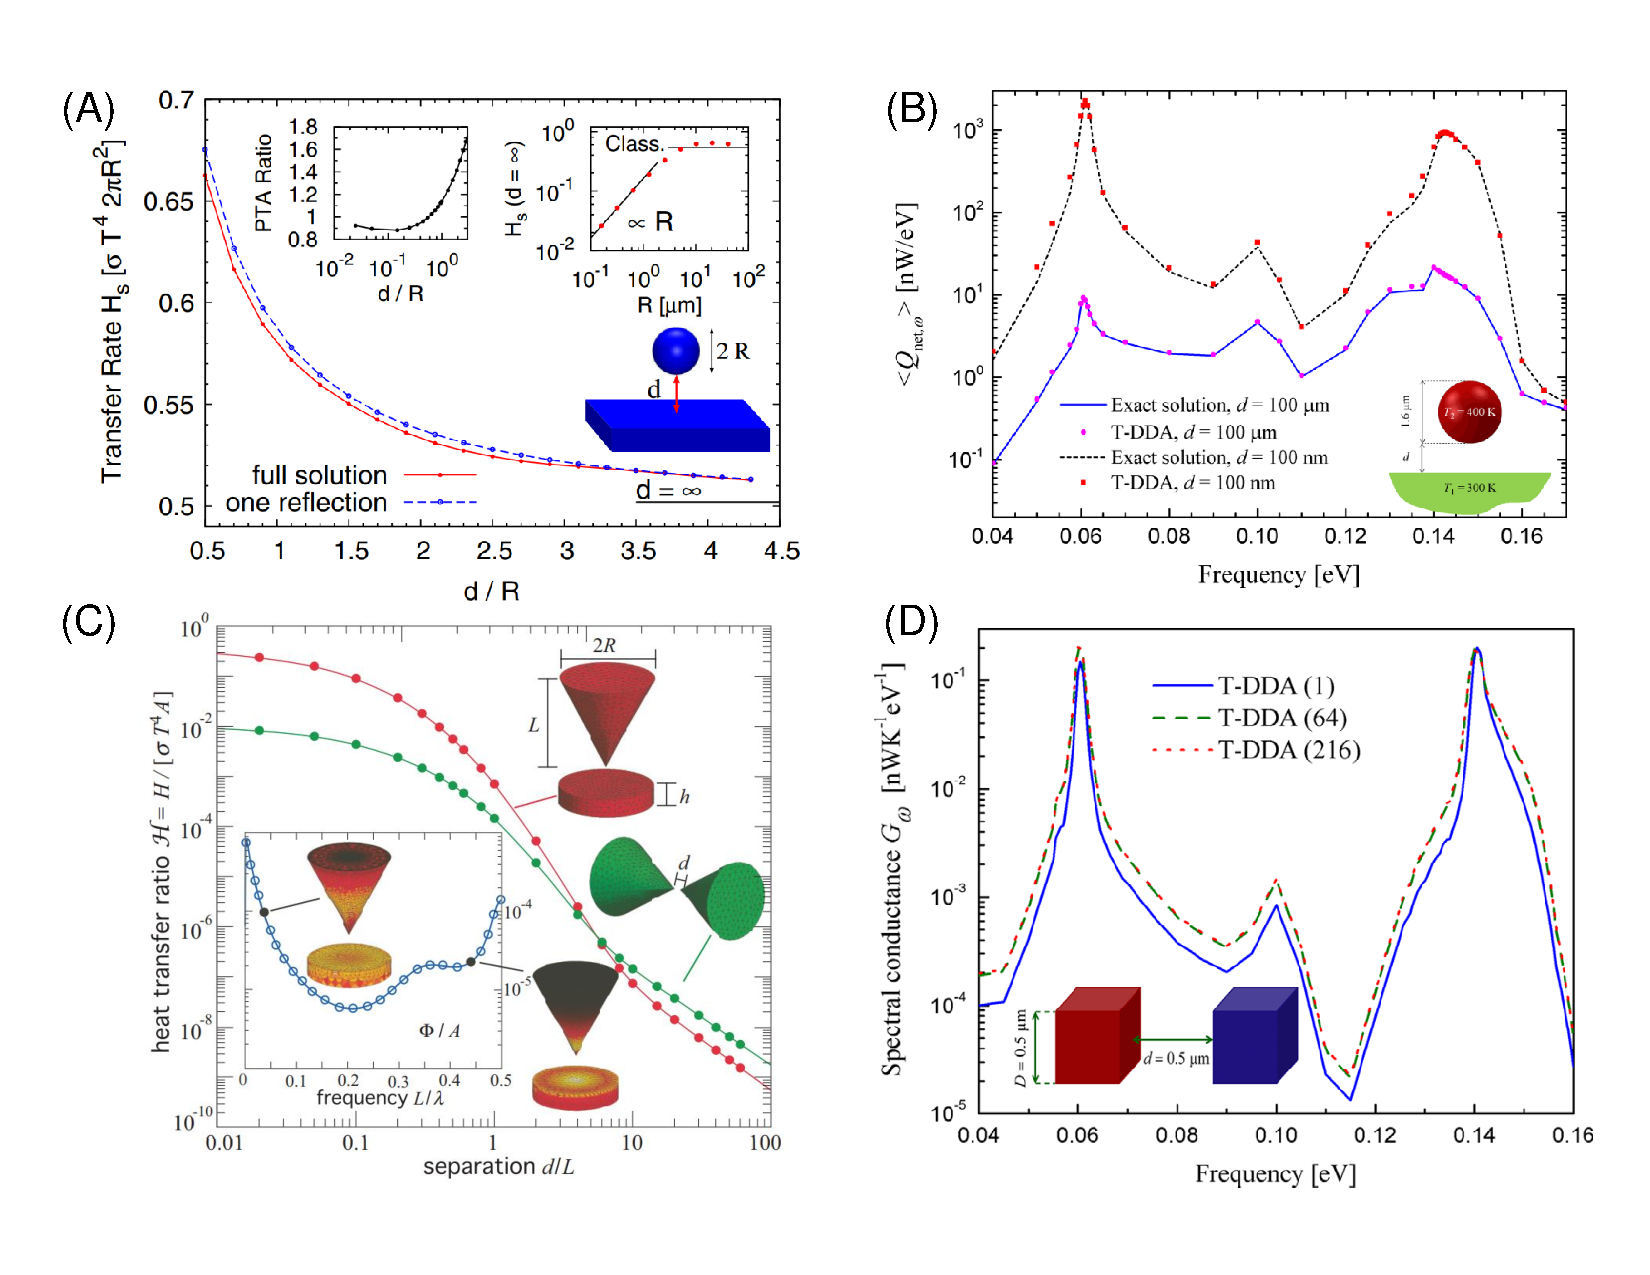
\includegraphics[width=\textwidth]{./Figures/ExactMethods.pdf}
\caption{\label{fig:ExactMethods}Selected NFRHT results from the literature. (A) Distance dependence of NFRHT in the sphere-plane configuration using spectral densities (labeled full solution).\cite{Kruger2011} (B) Frequency dependence of NFRHT in the sphere-plane configuration using DGFs (labeled exact solution) and T-DDA.\cite{Edalatpour2016} (C) Distance dependence of NFRHT in the cone-cone and cone-plane configurations using BEM.\cite{Rodriguez2013} (D) Frequency dependence of NFRHT in the cube-cube configuration using T-DDA.\cite{Edalatpour2014}}
\end{figure}


\subsection{Thermal Hyperbolic Metamaterials}
%
Optical metamaterials are a class of artificial materials which exhibit electromagnetic behavior not otherwise observed in nature, such as negative refractive index,\cite{Smith2004, Zhang2005, Soukoulis2007, Valentine2008} cloaking, \cite{Alu2005, Schurig2006, Cai2007, Valentine2009} and superlensing.\cite{Pendry2000, Fang2005, Smolyaninov2007, Zhang2008} Of particular interest are hyperbolic metamaterials (HMMs), materials whose permissible wavevector components form a hyperbolic isofrequency surface instead of the spherical surface found in typical isotropic materials. The simplest means of achieving HMM behavior is through layering different isotropic materials. When the layer thicknesses are much smaller than the free-space wavelength of light propagating through them, the entire nanocomposite can be viewed as a homogeneous material with hyperbolic effective optical properties.\cite{Halevi1999, Smith2003}

Hyperbolic metamaterials have found many uses in the field of near-field thermal radiative transfer. Appropriately designed HMMs have demonstrated the ability to tailor the spectrum of radiative transfer and to achieve super-Planckian heat transfer.\cite{Francoeur2011, Liu2011, Mason2011, Biehs2012, Guo2012, Guo2013, Liu2013} To date, this has mostly been achieved by using layered planar surfaces and computing the NFRHT using a DGF formalism.\cite{Biehs2007, Fu2009, Svetovoy2012} That configuration is attractive because the analytic solution to near-field thermal radiative transfer between two semi-infinite half spaces is well known, relatively straightforward to compute, and easily generalizes to include layered media.\cite{Polder1971, Francoeur2008, Francoeur2009, Song2016}

Figure \ref{fig:ExactMethods} depicts a typical numerical study of thermal HMMs.\cite{Guo2012a, Guo2013} Figure \ref{fig:ExactMethods}A shows two common methods of creating HMMs from linear, isotropic media. In this section, we focus on planar layered media. Figure \ref{fig:ExactMethods}B shows the spectrum of radiative transfer between two semi-infinite half spaces composed of alternating layers of silicon carbide and silicon dioxide. The left plot in Fig. \ref{fig:ExactMethods}B is obtained by integrating over the values of $k_{\rho}$ shown in the right plot. The main takeaway is that the contributions from high values of $k_{\rho}/k_{0}$, called high-k modes, are enabled by the hyperbolic optical properties of the half-spaces. 

HMMs composed of layered media are fundamentally limited in the extreme near-field. Mulet et al. showed that a particle exchanging thermal radiation with an object will only interact with the object to a depth comparable to the particle-object separation distance.\cite{Mulet2001} Considering any two layered objects to be made of an ensemble of particles, should the outermost layers become thicker than the separation distance, the near-field interaction should resemble NFRHT between two homogeneous objects composed of the outermost materials. This effect can lead to non-monotonic heat transfer with respect to distance.\cite{Esquivel-Sirvent2016}

\begin{figure}
\centering
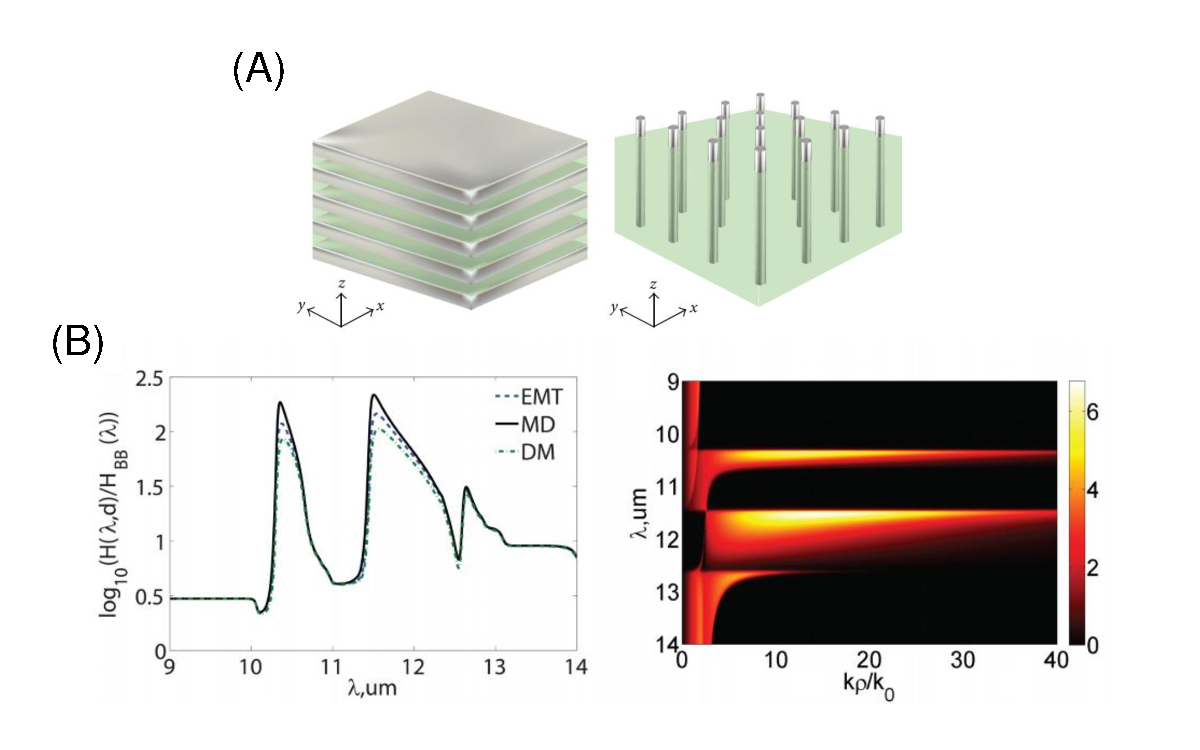
\includegraphics[width=\textwidth]{./Figures/HMM.pdf}
\caption{\label{fig:ExactMethods}(A) Schematic of two types of HMMs.\cite{Guo2012a} (B) Heat transfer between two layered semi-infinite half spaces composed of alternating layers of silicon carbide and silicon dioxide. The high-k modes are made possible by effective HMM optical properties.\cite{Guo2013}}
\end{figure}


\subsection{Experiments}
%
Compared to the great strides in theory made over the past decades, the experimental measurement of NFRHT is relatively immature. The oldest experiments involving NFRHT took place at between planar surfaces at cryogenic temperatures and relatively large gaps (10$^{2}$ \si{\micro\meter} to 10$^{3}$ \si{\micro\meter}).\cite{Cravalho1968, Domoto1970a} Though some modern work is still done at cryogenic temperatures\cite{Kralik2012} and/or using planar surfaces\cite{Kralik2012, Ghashami2018} (see Fig. \ref{fig:NFRHT_Experiments}C), most modern experiments occur at room temperature, and often do not involve two planar surfaces to avoid the difficulty in maintaining mutually parallel surfaces. Until the recent advances in NFRHT between MEMS devices\cite{Song2016, Cui2017, Fiorino2018} (see Fig. \ref{fig:NFRHT_Experiments}A), experiments measuring NFRHT in sub-micron gaps were performed in the microsphere-plane configuration (see Fig. \ref{fig:NFRHT_Experiments}B), much like the configurations used in Casimir and van der Waals force experiments.\cite{Lamoreaux1997, Mohideen1998, Roy1999, Harris2000} The rotational invariance of spheres, and to a lesser degree the small rotational variance of probes with rounded tips, removes the obstacle of maintaining parallel surfaces. A detailed critique of the microsphere-plane experimental configuration will be provided in Chapter \ref{ch:results}, based on the results of this dissertation.

\begin{figure}
\centering
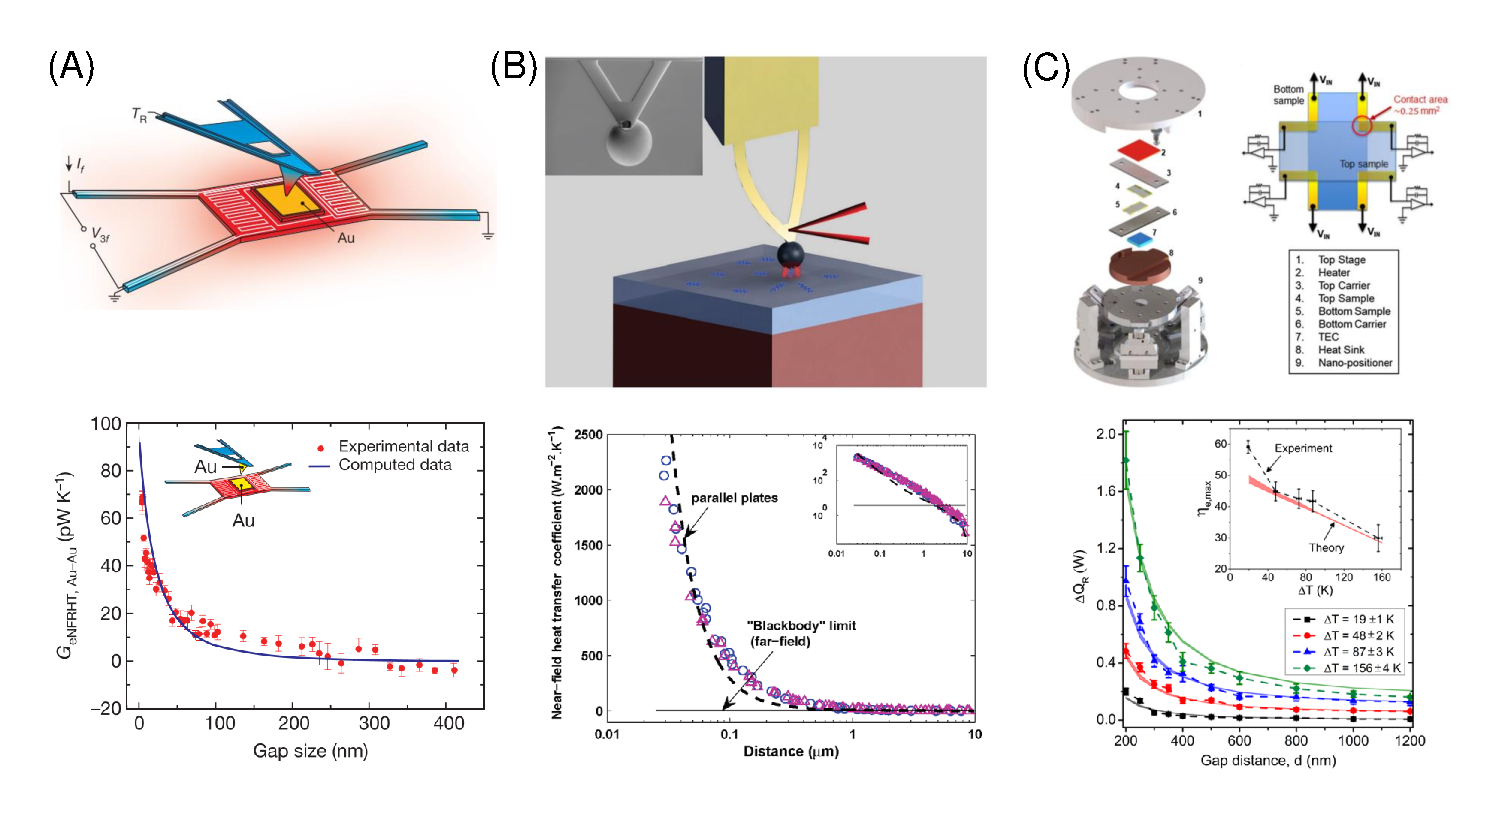
\includegraphics[width=\textwidth]{./Figures/NFRHT_Experiments.pdf}
\caption{\label{fig:NFRHT_Experiments}(A) NFRHT between a probe with a 300 \si{\nano\meter} radius spherical tip and a plane.\cite{Kim2015} (B) NFRHT between a sphere with a 50 \si{\micro\meter} or 100 \si{\micro\meter} radius and a plane.\cite{Shen2009} (C) NFRHT between two planar surfaces.\cite{Ghashami2018}}
\end{figure}


%\subsection{Open Questions}
%%
%Given the brief overview of NFRHT provided in this chapter, 
%
%What further geometries can be solved exactly?
%
%Extreme near-field, sub-Angstrom gaps. Radiation-condiction crossover, divergent bahviour of NFRHT isn't realistic, phonon tunneling, spatial dispersion
%
%Computation problems in many-body problems
%
%immature experiments compared to theory 
%
%Actual technologies


\section{Purpose and Outline of This Work}
%
The goal of this work is simple: to provide explicit formulas which completely describe a thermal system consisting of layered spheres in a linear chain. While this system has been previously investigated for two spheres,\cite{Narayanaswamy2008, Mackowski2008, Sasihithlu2011, Sasihithlu2011a, Kruger2012, Sasihithlu2012, Sasihithlu2014} light scattering,\cite{Fuller1988, Li2003, Wei2004, Chen2006, Lee2013} and radiative transfer in the dipole limit,\cite{Ben-Abdallah2011, Dong2017a, Kathmann2018} it has not yet been rigorously characterized for NFRHT between spheres of arbitrary size, with or without spherical layers. The key results of this work are numerically exact expressions for NFRHT between pairs of spheres in a linear chain, and between any sphere in a chain and its environment. The results of this dissertation allow for a rigorous critique of past sphere-plane experiments, focusing on how sphere-environment heat transfer is typically handled. Using the analysis, I provide a guidelines for designing future experiments between two spheres which ensure accurate interpretation of results. 

The outline of the dissertation is as follows: Chapter \ref{ch:Electromagnetism} builds up the basics of electromagnetic theory necessary to solve this problem. Starting from Maxwell's equations, the vector Helmholtz (wave) equation is derived for electric and magnetic fields in the Fourier domain. The Helmholtz equation is the governing equation for this work, and must be inverted to solve for the electric and magnetic fields, and ultimately radiative heat transfer. As part of that equation, knowledge of the optical properties of materials is required. I present a simple derivation of the Lorentz model for dielectric function and demonstrate how the model can be fit to a particular material by looking at a case study involving polydimethylsiloxane. Chapter \ref{ch:DGFs} covers the DGF formalism which will be employed to solve the problem. A general geometry for the formalism is established for an arbitrary number of objects embedded in a large free-space region. I show how DGFs can be used to isolate the contributions of fluctuating charges in each object to the electric and magnetic field at any other point. This will prove crucial to evaluating heat transfer between objects. I then go on to define the Poynting vector and describe the fluctuation-dissipation theorem, two important pieces to the puzzle. From there, I define a Landauer-like formula for radiative transfer that separates the temperature dependence from the geometric and configuration dependencies, which are contained in a transmissivity function for energy transfer. Crucially, the volumetric processes of emission and absorption are converted into surface integrals, which drastically simplifies computation. Finally, as a demonstration, I use the DGF formalism to compute NFRHT between planar media. Chapter \ref{ch:model} applies the DGF formalism to the case of coated spheres in a chain. The necessary eigenfunctions, the vector spherical waves, are provided which allow the DGFs of the system to be defined. The chain is analyzed and sphere-sphere and sphere-environment heat transfer formulas are provided. Chapter \ref{ch:results} serves to validate the results of this dissertation against BEM and T-DDA models before analyzing a few interesting cases. Those cases are NFRHT between two dielectric coated metal spheres and two dielectric coated dielectric spheres. I also propose a hypothetical two sphere NFRHT experiment and analyze the thermal model required to achieve accurate results. Chapter \ref{ch:Summary} summarizes my contributions to the field of NFRHT and suggests future areas of research.

Additionally, I supply a number of appendices for convenience of reference. Appendix \ref{ap:FresnelCoefficients} discusses the Fresnel reflection coefficients and provides their formulas. Appendix \ref{ap:CRT} is a brief summary of the common formulas used to compute CRT between two engineering surfaces. Appendix \ref{ap:Math} provides a number of mathematical formulas and relations useful throughout this work. Appendix \ref{ap:MieCoefficients} provides formulas for the effective Mie coefficients of layered media. Appendix \ref{ap:SolutionToLinearSystem} explains how to compute the scattered field coefficients that arise in sphere-sphere NFRHT calculations. Appendix \ref{ap:SCUFFEM} details the steps required to perform a NFRHT simulation using \textsc{scuff-em}.